\documentclass[11pt,a4paper]{article}
\usepackage{float}
\usepackage[utf8]{inputenc}
\usepackage[left=2cm,right=2cm,text={18cm,24cm},top=2cm]{geometry}
\usepackage[czech]{babel}
\usepackage{graphicx}
\usepackage{verbatim}
\usepackage{svg}
\usepackage{rotating}
\usepackage{hyperref}

\renewcommand{\familydefault}{\sfdefault}

\begin{document}
\begin{titlepage}
	\begin{center}
		% FIT logo
		
\includegraphics[scale=0.65]{img/fit.pdf} \\
				
		\vspace{2cm}
		
		\Large{
			IMP 2023/24
		}
						                
		\vspace{2cm}
\vspace{2cm}


  
		\huge{
			\textbf{
		Projektová dokumentace}}
		\vspace{2cm}
		\\
		      
		\huge{
			\textbf{
				ESP32: Měření srdečního tepu \\
				digitální senzor } \\}
				
							                
			\vspace{2cm}

			\Large{}
			\today{}
			
			\vspace{2cm}
			
			Matyáš Strelec \verb|xstrel03|
			\end{center}
			\end{titlepage}
			
        \pagebreak{}
			
        \tableofcontents
			
        \pagebreak{}

         \section{Úvod}

            Cílem projektu bylo vytvořit funkční sensor tepu se zobrazením hodnot na displeji pomocí desky ESP32.

            Projekt se založen na vývojové desce Wemos D1 s SoC ESP32, ke které je připojen sensor srdečního tepu MAX30102
            \cite{hwkitchen-max30102} a OLED displej SSD1306 \cite{hadex-ssd1306}.

            Projekt je implementován v jazyce C++, s pomocí editoru VS Code a jeho rozšíření PlatformIO. Pro práci se zařízeními
            je užito těchto knihoven:
            
            \begin{itemize}
                \item \verb|Adafruit_SSD1306| \cite{github-ssd1306}, 
                \item \verb|Adafruit-GFX-Library| \cite{github-gfx}
                \item \verb|SparkFun_MAX3010x_Sensor_Library| \cite{github-max3010x}
            \end{itemize}
            
            \subsection{Zapojení}

            Na desku Wemos D1 založené na ESP32 je připojen displej SSD1306 přes rozhraní SPI a senzor tepu MAX30102 přes rozhraní
            SPI. Obě komponenty jsou napájeny napětím 3.3 V.

            \begin{figure}[ht]
        		\centering
        		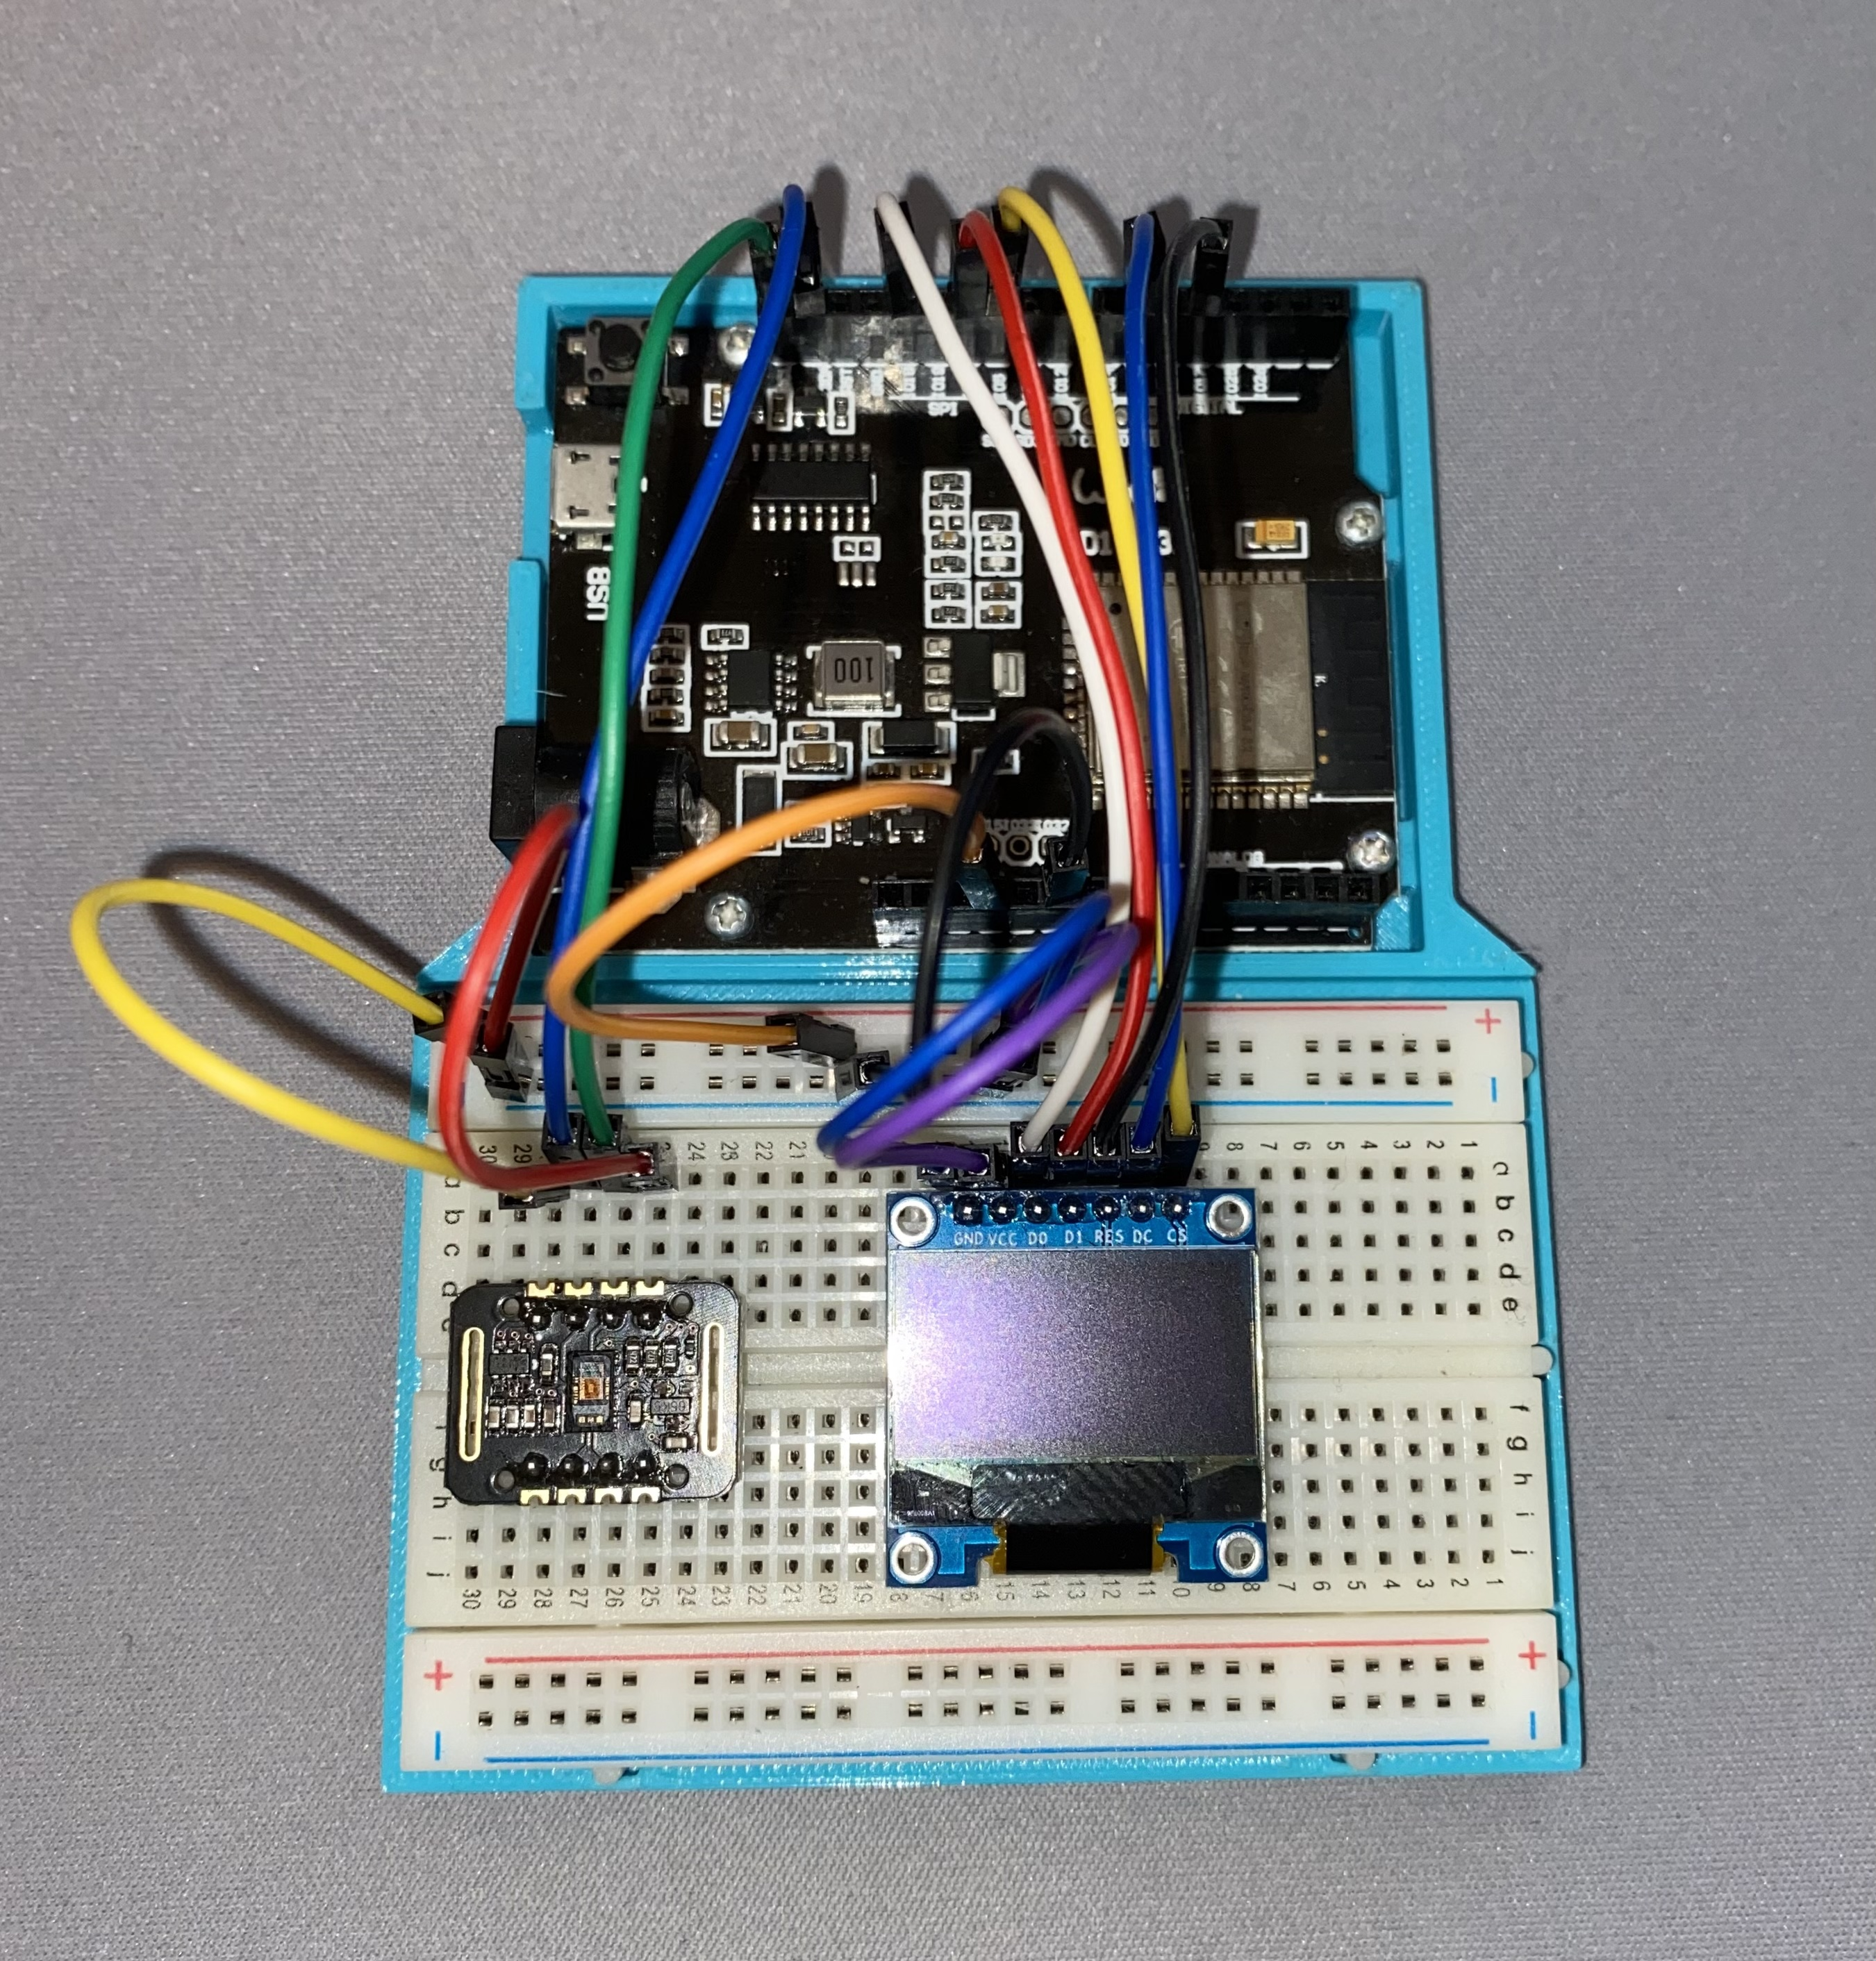
\includegraphics[width=0.6\linewidth]{img/zapojeni.jpg}
        	    \caption{Detail zapojení desky}
            \end{figure}
                    
            \subsection{Spuštění}

            Projekt lze spustit ve Visual Studio Code s nainstalovaným rozšířením Platformio\cite{pio}. Stačí založit nový
            projekt, vybrat desku Wemos D1 a naimportovat knihovny a zdrojové soubory. Pro nahrání do zařízení a spuštění
            lze použít funkce Upload \& Monitor.

        \section{Implementace}

            \subsection{Soubor \texttt{heartrate.cpp}}

            Soubor obsahuje hlavní kód celého programu.
   
                \subsubsection{Funkce \texttt{setup}}

                Funkce se spustí poprvé, při zapnutí zařízení. Inicializuje výstup do konzole, sensor tepu a displej. Sensor je 
                inicializován s výchozími hodnotami, kromě intenzity svitu LED diody, který je od výchozích slabší. Při moc
                silné intenzitě byl sensor méně přesný.

                Je zde nastaven také font, kterým se tiskne na displej. Při spuštění se zobrazí text "Heart rate monitor" a 
                přehraje se krátká animace tlukotu srdce.
    
                \subsubsection{Funkce \texttt{loop}}

                Hlavní smyčka programu, která se neustále opakuje. Z hodnoty přečtené z infračerveného sensoru se pomocí funkce
                \verb|checkForBeat| zjistí, zda-li je validní hodnotou tepu.

                Pokud ano, vypočte se delta $\Delta t$ od posledního zachyceného tepu a pomocí vztahu $BPM = \frac{60}{\Delta t / 1000}$ se vypočte počet tepů za sekundu.
                
                Do pole pro průměrné hodnoty se ukládají pouze reálné hodnoty, tedy ty mezi 40 a 200 tepy
                za minutu. Všechny tyto hodnoty se aritmeticky zprůměrují.

                Pokud sensor přečte nízkou hodnotu, znamená to, že prst je moc daleko od sensoru, vyzve tedy k přiložení. V
                opačném případě vypíše hodnoty naměřené jak do konzole, tak na displej. 
    
                \subsubsection{Funkce \texttt{printPlaceFinger}}

                Funkce periodicky na displeji zobrazuje text "Place finger on sensor" a ikonku otisku prstu. Tyto dvě obrazovky
                se každou sekundu obmění.
    
                \subsubsection{Funkce \texttt{printHeartRate}}

                Funkce dostává parametrem hodnoty aktuálního a průměrného tepu, které má na displeji vykreslit. Kromě toho
                vedle hodnot tepu vykresluje animaci tlukoucího srdce.
    
            \subsection{Soubor \texttt{images.h}}

            Tento soubor obsahuje definice obrázků zobrazených na displeji, konkrétně 2 obrázky pro animace tepu srdce a 1 obrázek
            pro otisk prstu. Tyto obrázky byly nakresleny digitálně a převedeny do bajtů pomocí webového nástroje\cite{mischianti}.
            
        \section{Ukázka}
			
            \subsection{Video}

            Pro účely demonstrace funkčnosti projektu jsem nahrál krátké video, které lze shlédnout na YouTube na
            tomto odkaze: \url{https://www.youtube.com/watch?v=c5osdgcbPcA}. 
            
        \section{Závěr}

            Projekt byl zajímavým exkurzem do programování desky ESP32. Zkoumáním knihoven a článků jsem na řešení přišel
            poměrně jednoduše, správné zapojení bylo také zvládnutelné. Získání přesných měření ze sensoru je trochu oříšek,
            protože požaduje velmi jemné zacházení a přesné držení prstu, ze kterého snímá tep, jinak z něj nejde přečíst
            smysluplná hodnota. Při úspěšném měření jsem jej validoval proti sensoru tepu na hodinkách Apple Watch SE, kde
            rozdíl v hodnotě byl v rámci 10 \%, lze tedy říci, že má implementace měří přesně.
           
            \subsection{Autoevaluace}

                Celkové hodnocení ($\Sigma$) je dáno vztahem $\Sigma = (K_1 + K_2 \cdot F/5) \cdot (E + F + Q + P + D)$

                \subsubsection*{Konstanta $K_1 = 0.25$}
                \subsubsection*{Konstanta $K_2 = 0.75$}
                
                \subsubsection*{Přístup $E = 1$}

                Na projektu jsem začal pracovat včas, měl jsem problém s nefunkčním dodaným senzorem, který jsem mohl včas
                vyřešit. Snažil jsem se o kvalitní projekt, implementace je funkční, zároveň jsem se snažil o hezkou vizuální
                stránku zobrazení dat s obrázky a animacemi ikon tepu nebo přiložení prstu.

                \subsubsection*{Funkčnost $F = 5$}

                Cílem zadání je funčkí snímač tepu senzoru se zobrazením na displeji. Má implementace toto splňuje, měří
                aktuální tep i počítá průměrný, tyto hodnoty zobrazuje na displeji.

                \subsubsection*{Kvalita $Q = 3$}

                Uživatelská přívětivost je vysoká, stačí zapojit dle části 1.1, vytvořit nový projekt, kód nahrát do zařízení
                dle části 1.2 a projekt běží. Zdrojové kódy jsou přehledné, psané jednotně, naformátované a patřičně okomentované.
                Kód je v jednom souboru, jelikož mi nedává smysl takto krátký projekt rozdělovat. Je ale rozdělen na podproblémy,
                které řeší jednotlivé funkce.

                \subsubsection*{Prezentace $P = 1$}

                Video zobrazuje veškerou funkcionalitu v co nejkompaktnějším podání.

                \subsubsection*{Dokumentace $D = 4$}

                Dokumentace je graficky i typograficky kvalitně zpracovaná a vysázená, po informační stránce obsahuje vše,
                co by měla, jako úvod, popis implementace, ukázku, a závěr.

                \subsubsection*{Výsledek $\Sigma$}

                Celkové hodnocení dle autoevaluace je tedy $\Sigma = (0.25 + 0.75 \cdot 5/5) \cdot (1 + 5 + 3 + 1 + 4) = \mathbf{14}$.

	\clearpage

 	\renewcommand{\refname}{Zdroje}

	\bibliographystyle{doc/czechiso}
 	\bibliography{doc/sources}
 
\end{document}
